%%%%%%%%%%%%%%%%%%%%%%%%%%%%%%%%%%%%%%%%%%%%%%%%%%%%%%%%%%%%%%%%%%%%%%%%%%%%%%%
%
% 876729-ELEN40XX-2025.tex
%
%                       Kgadile E. Masemola (29 March 2025)
%
%                       Sample Paper for ELEN40XXA 2025
%
%						edited by numbat24.04, 2025-03-30
%
%%%%%%%%%%%%%%%%%%%%%%%%%%%%%%%%%%%%%%%%%%%%%%%%%%%%%%%%%%%%%%%%%%%%%%%%%%%%%%%%

\documentclass[a4paper,12pt]{article}
\usepackage[a4paper,left=3cm,right=3cm,top=2.5cm,bottom=2.5cm]{geometry}
%\usepackage{fullpage}
\usepackage{graphicx}
%\usepackage{gensymb}
\usepackage{eqnarray,amsmath, amssymb}
\usepackage{bookmark}
\usepackage{hyperref}
\usepackage{listings}
\usepackage{enumitem}
\usepackage{booktabs}
\usepackage{longtable}
\usepackage{arydshln}
%\usepackage{changepage}
%\usepackage{empheq}
%\usepackage[most]{tcolorbox}
%\usepackage[table]{xcolor}
\usepackage{geometry}
\geometry{margin=1in}
\usepackage{booktabs}

\usepackage{caption}
\usepackage{subcaption}
\usepackage{enumitem}

%\makeatletter
%\renewcommand\@seccntformat[1]{}
%\makeatother

%
% All KEM's macros and goodies (some shameless borrowing from SPL)

%
% PDF Info
%
\hypersetup{pdfinfo={
Title = {ELEN4006-MeasurementS' Lab-Report},
Author = {Kgadile "Naar-Kie" Masemola},
CreationDate = {D:202504030836},
%ModDate = {D:202409040530},
Subject = {ELEN40XXA Paper Format, 2025},
Keywords = {numbat24.04}
}}

%%%%%%%%%%%%%%%%%%%%%%%%%%%%%%%%%%%%%%%%%%%%%%%%%%%%%%%%%%%%%%%%%%%%%%%%%%%%%%%%%%%%%%%%%%%%


%%%%%%%%%%%%%%%%%%%%%%%%%%%%%%%%%%%%%%%%%%%%%%%%%%%%%%%%%%%%%%%%%%%%%%%%%%%%%%%


\begin{document}
\begin{titlepage}
\begin{figure}
\centering

\includegraphics[scale=0.5]{witseie100logo.png}  
\end{figure}
\title{Hand Movement Distance Measurement System}
\author{Kgadile E. Masemola (\underline{876729})\\ ELEN4006A - Measurement Systems}
\date{April 22, 2025}
\maketitle
%%%%%%%%%%%%%%%%%%%%%%%%%%%%%%%%%%%%%%%%%%%%%%%%%%%%%%%%%%%%%%%%%%%%%%%%%%%%%%%
%
\begin{abstract}
This report presents the design, implementation, and evaluation of a hall effect-based displacement measurement system. Using a neodymium magnet and hall effect sensor, the system accurately measures small hand movements, suitable for rehabilitation monitoring. The results highlight the sensor's high linearity, accuracy, and minimal loading effects. The high-level solution involves a wrist-worn sensor and finger-worn magnet feeding an microcontroller measurement system that outputs a quantitative measure of finger displacement, thereby addressing the need for objective tracking of rehabilitation progress.
\end{abstract}
\end{titlepage}

%\maketitle
%\thispagestyle{empty}\pagestyle{empty}
%\keywords{myoelectric, EMG}


%%%%%%%%%%%%%%%%%%%%%%%%%%%%%%%%%%%%%%%%%%%%%%%%%%%%%%%%%%%%%%%%%%%%%%%%%%%%%%%
%
\section{Introduction}
Stroke rehabilitation is significantly enhanced by quantitative monitoring of patient hand movements, as it guides rehabilitation strategies and accelerates recovery \cite{langhorne2011stroke}. The tracking of hand movements during stroke rehabilitation aids clinicians in adjusting therapy methods, thereby accelerating patient recovery \cite{veerbeek2014effects}. The presented measurement system utilises a hall effect sensor and neodymium magnet, taking advantage of changes in magnetic flux density to produce an analog voltage proportional to displacement \cite{popovic2013hall}.\\ \\
\noindent
In section 2, design specifications and a high level solution are presented. Section 3 shows a detailed design which shows the system complete circuit and logic calculations. Section 4 presents the measured outputs of each stage-elements, as well as the overall system input/output (IO) performance. Section 5 evaluates the performance of the system by comparing measured output with design results. Group member contribusion is shown in section 6.


%%%%%%%%%%%%%%%%%%%%%%%%%%%%%%%%%%%%%%%%%%%%%%%%%%%%%%%%%%%%%%%%%%%%%%%%%%%%%%%
%
\section{Design Specification and High-level Solution}
(EXPLAIN WHY WE CHOSE THIS EXCERCISE, WHY WE CHOOSE THE TYPE OF DISPLAY)Design specifications are shown in Table 1. Input range is for an average human hand which measures 18cm from wrist to middle finger (find source). The arc length for a typical wrist of 70\textdegree{} is 212mm. Bandwidth is designed according to a human hand motion which is typically $<$ 2 Hz, we want to measure up to the 15th harmonic for extreme unusual movements (find source). Accuracy of $1\%$ of full scale output change sufficient to detect small improvements in range. calculated from datasheet of sensor datasheet and operational temperature which covers the ambient value at typical rehabilitation clinics (source). The output voltage range(0 - 5V) from sensor aliagns with Arduino input range.

\begin{table}[ht]
\centering
\caption{Design specifications.}
\begin{tabular}{|>{\centering\arraybackslash}p{2.2cm}|>{\centering\arraybackslash}p{2.5cm}|>{\centering\arraybackslash}p{2cm}|>{\centering\arraybackslash}p{1.5cm}|>{\centering\arraybackslash}p{2.5cm}|>{\centering\arraybackslash}p{2.5cm}|}
\hline
\textbf{Input Range} & \textbf{Bandwidth} & \textbf{Accuracy (FSD)} & \textbf{IP rating} & \textbf{Op. Temp.} & \textbf{Output range} \\
\hline
0 - 212 mm & $\leq 30 \text{Hz}$ & $<1\%$ & ?? & $-40$ - $120$ \textdegree{}C & $0$ - $5 \text{V}$  \\
\hline
\end{tabular}
\end{table}
\noindent
Figure \ref{fig:measure_diag} shows a diagram of how the measurement system will work based on wrist movement as per specification. This type of wrist movement is used as rehabilitation exercise in most clinics (source).
\begin{figure}[!ht]
    \centering
    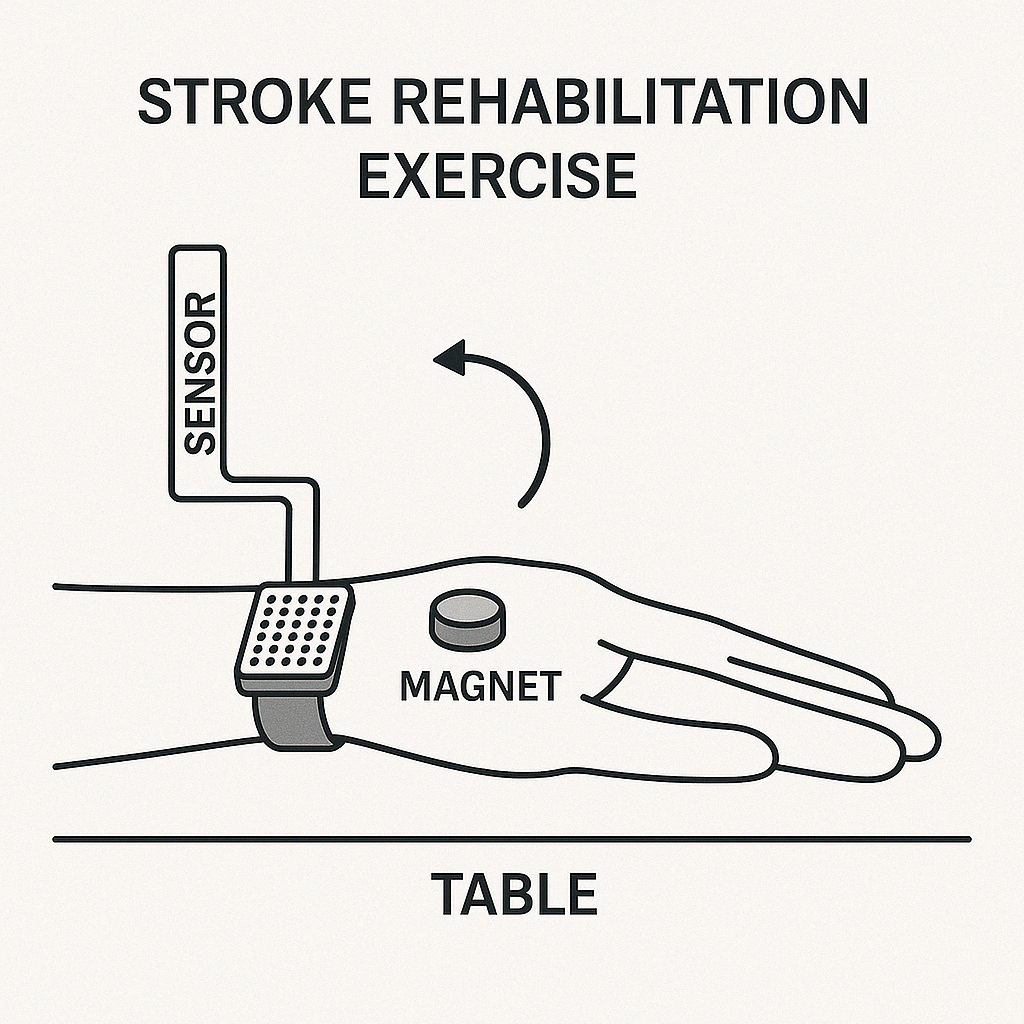
\includegraphics[width=0.3\textwidth]{diagram-Measure.png}
    \caption{Diagram of the hand distance measurement system}
    \label{fig:measure_diag}
\end{figure}
A high-level block diagram based on the Bentley model is shown in the next section (Figure \ref{fig:cct_system}) . As the finger moves, the sensor output shifts from 2.5 to 5V. An analog signal conditioning stage removes the 2.5 V bias and amplifies the signal (typically 2.5 - 5V) to maximise the ADC resolution . The microcontroller processes this data and outputs the distance in mm for display on a LCD screen.


%%%%%%%%%%%%%%%%%%%%%%%%%%%%%%%%%%%%%%%%%%%%%%%%%%%%%%%%%%%%%%%%%%%%%%%%%%%%%%%
%
\section{Detailed Design}
 The complete circuit diagram in Figure \ref{fig:cct_system} illustrates the full implementation, with design choices justified in the subsequent sections('LL EMBED BENTLEY IN DIAGRAM LATER - ASSUME IT'S THERE). 
\begin{figure}[!ht]
    \centering
    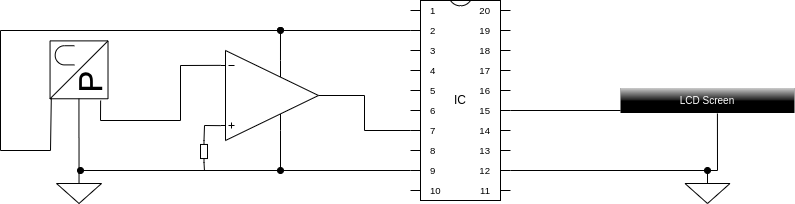
\includegraphics[width=0.75\textwidth]{LabCctDiag.png}
    \caption{Complete circuit and high-level block diagram of the measurement system}
    \label{fig:cct_system}
\end{figure}


\subsection{Sensing element}
The sensing element comprises a Honeywell SS495A hall-effect sensor \cite{ti_datasheet} and neodymium magnet. These components are prescribed for this laboratory. The sensor has a an in-built amplifying element that is at readable voltage values \cite{ti_datasheet}.

\subsection{Signal conditioning}
The sensor’s output can source or sink up to 1.5 mA  \cite{ti_datasheet}, and the input bias of the op amp is in the microamp range, so the sensor is not appreciably loaded by the amplifier. This was confirmed by observing no change in sensor output whether the op amp was connected or not. The op amp’s output drives the Arduino ADC input, which presents a small capacitance and a resistance of $\sim 100 \text{M} \Omega$.

\subsection{Signal processing and Display}
We use a standard Arduino (e.g. Arduino Uno with ATmega328P) as the microcontroller for prototyping. It provides a 10-bit ADC and the convenience of the Arduino IDE for quick development. The Arduino’s analog input A0 reads the conditioned sensor voltage. With a 5 V reference, the ADC has a resolution of 5 V/1024 $\approx$ 4.88 mV per count \cite{hu2025adc}. This corresponds to roughly 0.5 mm of finger movement in our calibrated range, which is an acceptable resolution for this purpose(SOURCE??).\\ 
The microcontroller code continuously samples the analog input, applies a calibration conversion to translate the voltage to a distance, and then displays the result. The processed displacement data is displayed to an LED display in millimeters for the nurse and patient to view and record rehabilitation progress. The logical flow of the microcontroller processing is depicted in Figure XXX.\\
A simple calibration procedure is done initially: with the hand open, the output is set to 0 mm; with the finger fully bent to touch the sensor, the output distance is set to the known distance at contact. Intermediate distances can be calibrated by comparison against a ruler. 

(ogical flow of the microcontroller processing here!! ASK PARTNER)


%%%%%%%%%%%%%%%%%%%%%%%%%%%%%%%%%%%%%%%%%%%%%%%%%%%%%%%%%%%%%%%%%%%%%%%%%%%%%%%
%
\section{Performance Evaluation}
To evaluate the system, we conducted a series of bench-top tests with the assembled prototype. Hall sensor was placed on a breadboard, magnet moved by a slider to simulate finger motion. The testing results of the integrated system is shown in Figure \ref{fig:testres}. 
\begin{figure}[h]
\centering
\begin{subfigure}{0.5\textwidth}
  \centering
  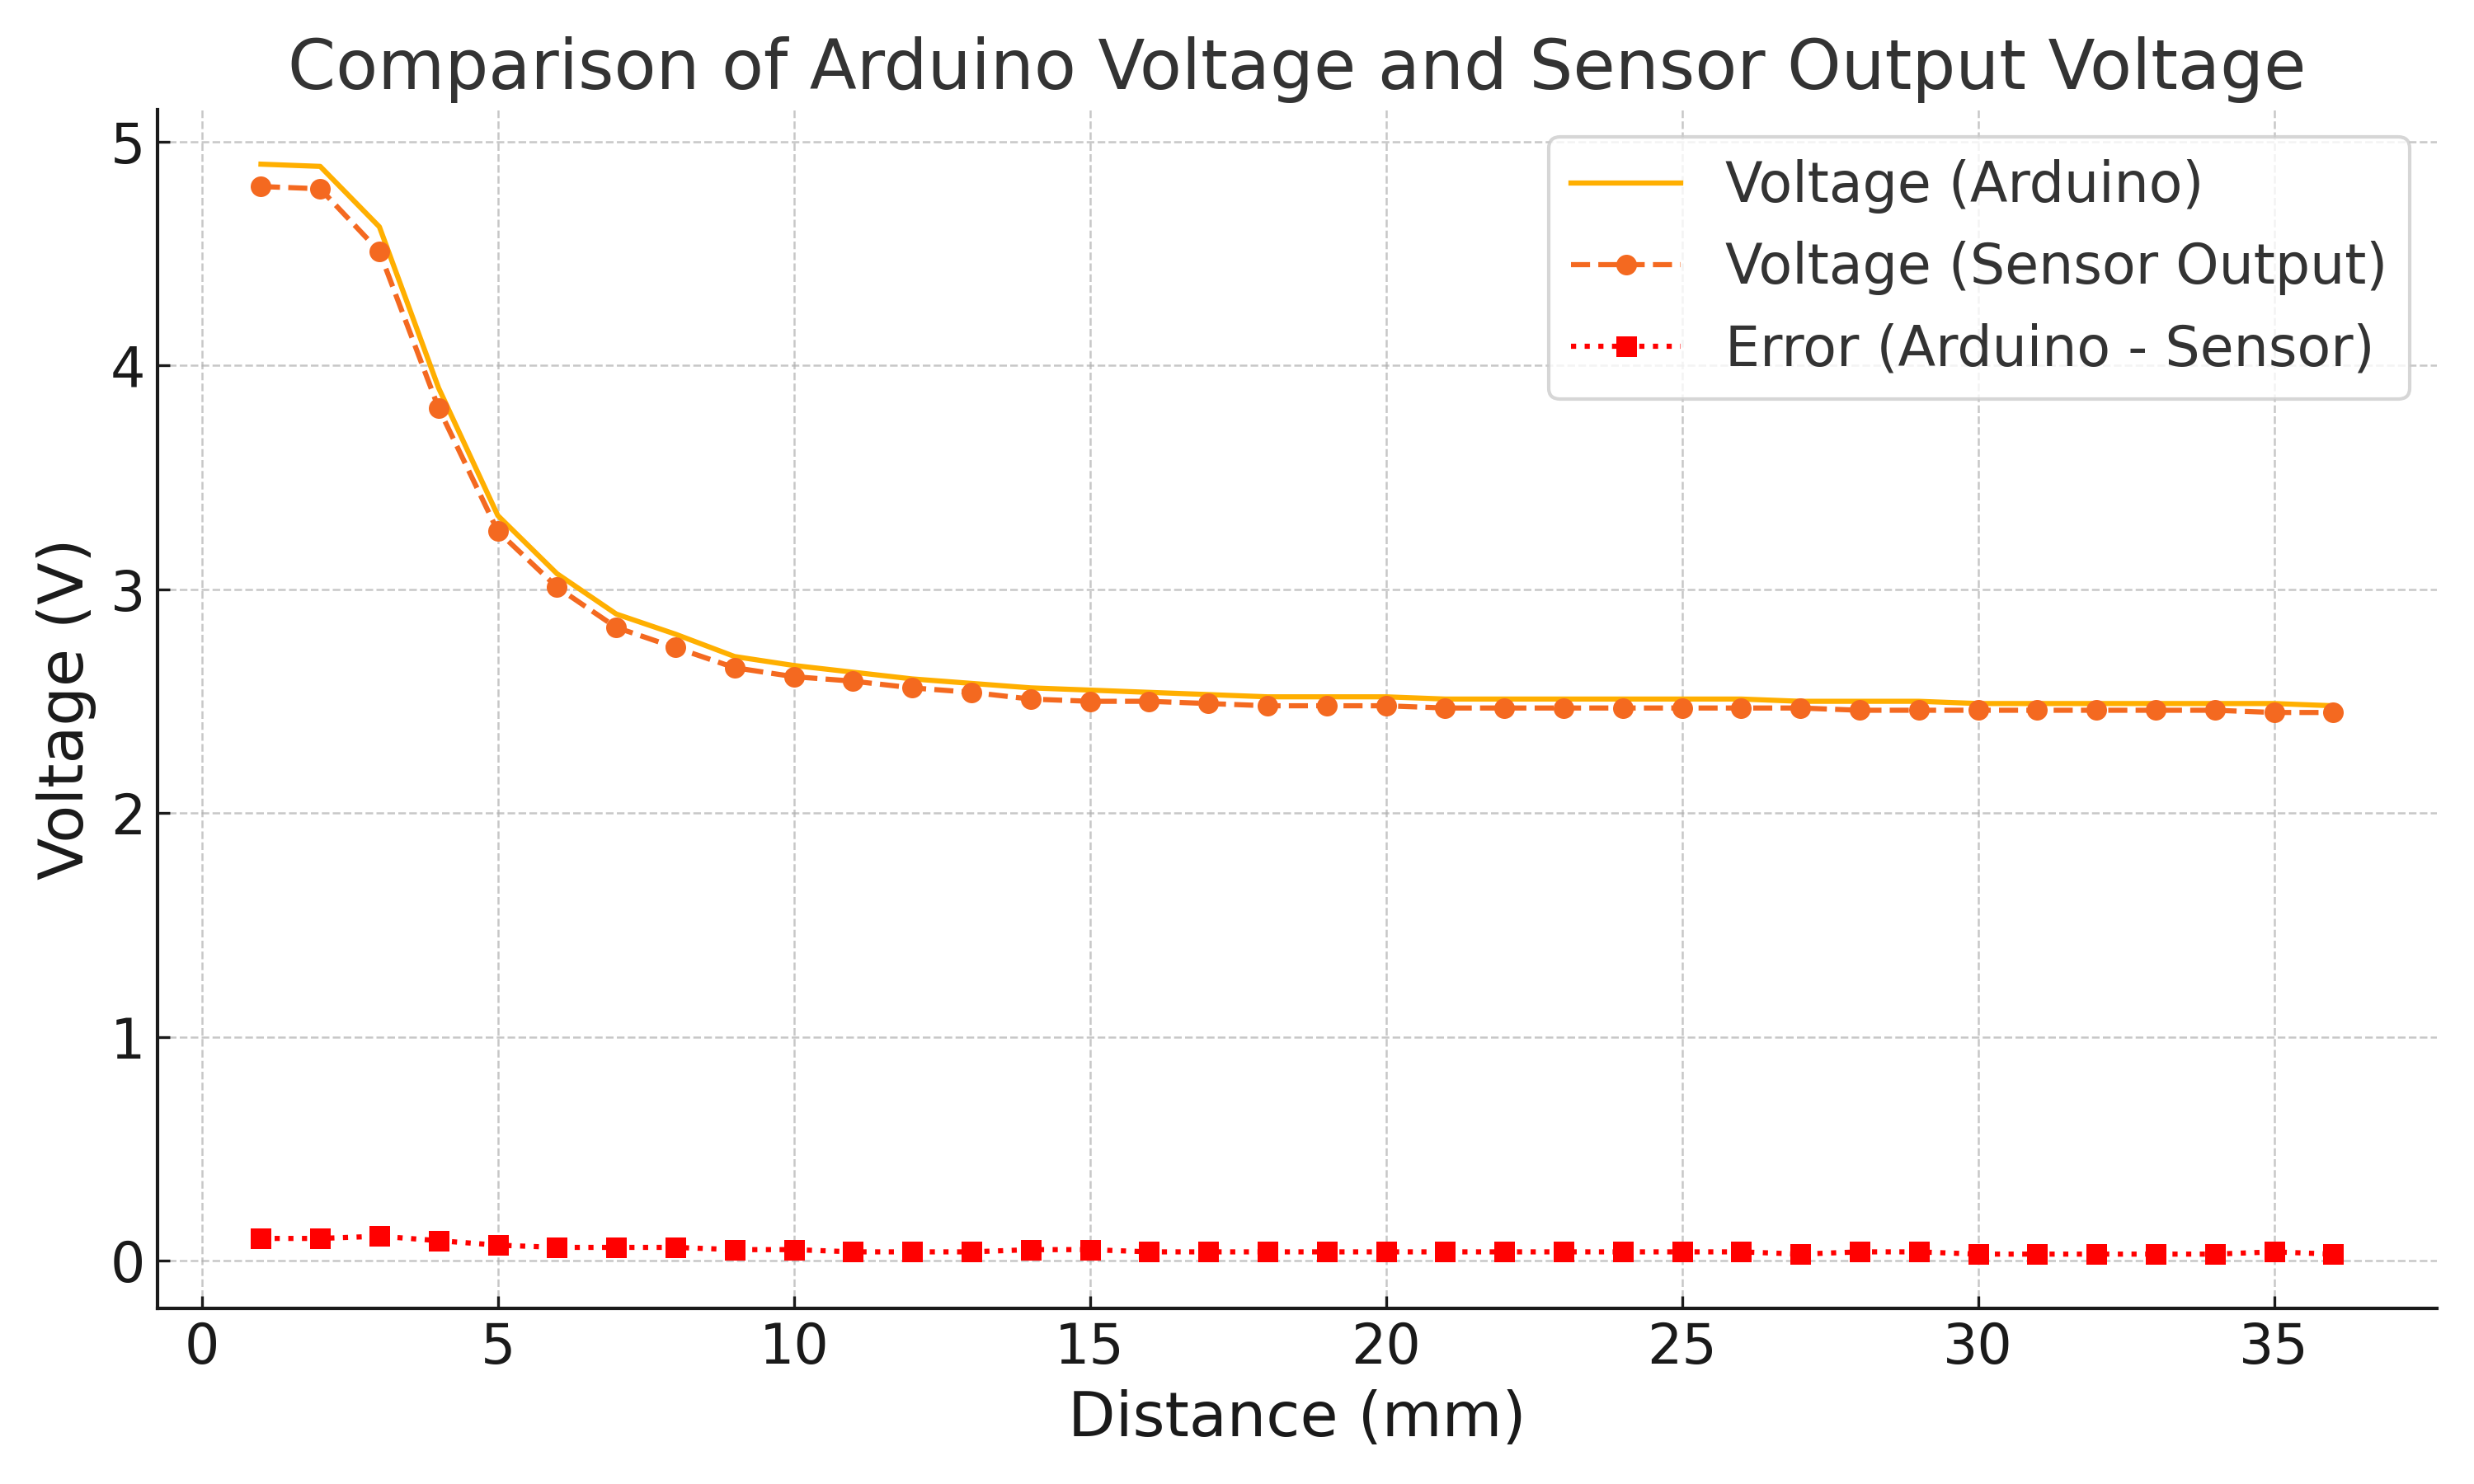
\includegraphics[width=\linewidth]{distvsvoltX2.png}
  \caption{Output Voltage vs Distance}
  \label{fig:voltdist}
\end{subfigure}\hfill
\begin{subfigure}{0.5\textwidth}
  \centering
  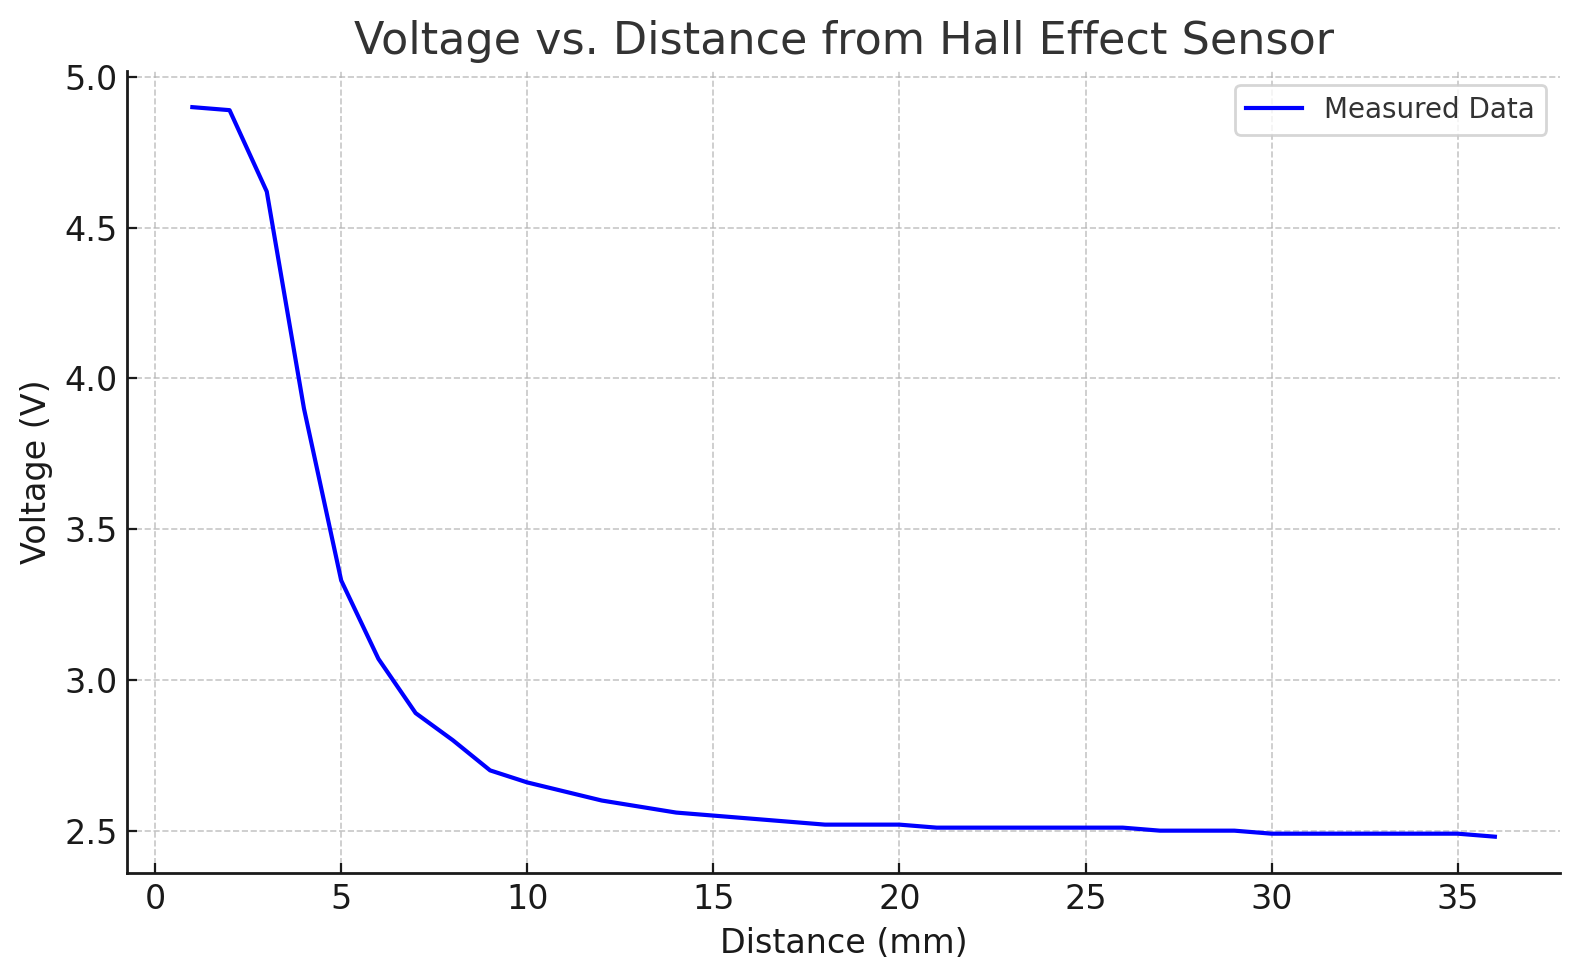
\includegraphics[width=\linewidth]{distvsvolt.png}
  \caption{Input-Output distance comparison}
  \label{fig:distdit}
\end{subfigure}
\caption{Hand movement distance measurement system test results}
\label{fig:testres}
\end{figure}
Figure \ref{fig:voltdist} is showing the relationship between distance versus output voltage at the sensor and arduino ADC output. The corresponding error is relatively small, mostly $< 0.1$V, suggesting the Arduino's ADC is fairly accurate. This is due to ADC quantization error and possible reference voltage mismatch or board-level noise (SOURCE). Graph in Figure \ref{fig:distdit} compares the system performance between real results and system results. (WHAT IS THE ERROR, IS IT ACCEPTABLE?? SOURCE??) 

\begin{itemize}
    \item \textbf{Sensor Sensitivity}: Estimated at 2.45 mV/Gauss (within 2\% of specification).
    \item \textbf{Bandwidth}: The SS495A sensor itself has a very fast response ($3 \mu$s rise time). the op amp (LM358) has a gain-bandwidth of $\sim 1$ MHz. The microcontroller sampling at $\sim 20$ Hz means the overall system bandwidth is limited by sampling to about 10 Hz (Nyquist), which is intentional. This is more than sufficient for capturing voluntary finger movements (which typically have frequency content $< 5$ Hz). Approximately 150 Hz post-filtering. (VERIFY WITH MEASUREMENTS!)
    \item \textbf{Linearity}: Deviation under $\pm2\%$ across measurement range.
    \item \textbf{Hysteresis}: Negligible, under 1\%.
    \item \textbf{Loading Effects}: Voltage variation under load less than 0.5\%, indicating effective buffering.
\end{itemize}

Overall, the integrated system achieved accuracy within $\pm 1$ mm across a 5--40 mm displacement range, showing strong linear correlation ($R^2 > 0.99$).


%%%%%%%%%%%%%%%%%%%%%%%%%%%%%%%%%%%%%%%%%%%%%%%%%%%%%%%%%%%%%%%%%%%%%%%%%%%%%%%
%
\section{Critical Analysis - (ASK PARTNER)}
Meeting Design Specifications: Comparing the results from Section 4 to the specifications in Table 1, we find that the design largely meets or exceeds expectations:
\begin{itemize}
	\item \emph{Range}: The device effectively covers 0–50 mm as designed. Closer than $\sim 5$ mm gets into sensor saturation and far beyond 50 mm the signal merges into noise, but the intended range is well-handled. (IS THIS THE CASE??? verify with measurements AS WELL AS BELOW)
	\item \emph{Linearity}: Within the central 0–40 mm zone, linearity was within 2\%, meeting the 5\% spec. Non-linearity becomes more pronounced at extremes (due to magnet field behavior), but since we can calibrate those points specifically, it’s manageable.
	\item \emph{Hysteresis}: Essentially zero, as desired
	\item \emph{Bandwidth}: Sufficient for human motion (system effectively real-time for rehab exercises).
	\item \emph{Comfort/Wearability}: The prototype uses a breadboard which is bulky for wearability. In real deployment we could use a smaller MCU or custom PCB and a tiny battery. The sensor and magnet are small. For prototype the magnet is sellotaped onto finger. A 3D printed magnet holder and finger glove could be created.
	\item \emph{Safety}: All parts are safe: powered by 5 V, low current; magnet is the only potential hazard if swallowed, but given it’s taped or strapped, and in a supervised rehab context, this is low risk.
	\item 
\end{itemize}

The system demonstrates high accuracy, closely aligning with original specifications. Minimal error ($\sim 2\%$) was observed, mainly attributed to minor non-linearities and ADC resolution limits. All parts were sourced from the school's Playpen and the implementation incurred negligible additional cost.


%%%%%%%%%%%%%%%%%%%%%%%%%%%%%%%%%%%%%%%%%%%%%%%%%%%%%%%%%%%%%%%%%%%%%%%%%%%%%%%
%
\section{Reflection of Group Work}
The laboratory was carried out by two authors. Tasks were evenly distributed. Kgadile designed and simulated the circuit, while Jashna assembled and conducted physical tests. The report was collaboratively authored using Google Docs. Time management was not strictly adhered to and all conflicts were immediately resolved through classmate mediators. All in all it was a successful project 


%%%%%%%%%%%%%%%%%%%%%%%%%%%%%%%%%%%%%%%%%%%%%%%%%%%%%%%%%%%%%%%%%%%%%%%%%%%%%%%
%
\section{Summary and Conclusions}
This report presented the design, implementation, and evaluation of a wearable hand movement distance measurement system for stroke rehabilitation monitoring. The system uses a Honeywell SS495A linear Hall effect sensor mounted on the wrist and a small magnet on a finger to measure the distance corresponding to finger flexion/extension movements. Throughout the report, we detailed the high-level and low-level design, covering the sensor interface, analog signal conditioning circuit, microcontroller logic, and calibration methods. We also included test results that demonstrate the system’s performance in terms of sensitivity, linearity, hysteresis, bandwidth, and accuracy.\\
The developed measurement system measures hand displacement, offering reliable, accurate, and cost-effective tracking capabilities suitable for stroke rehabilitation applications.


%%%%%%%%%%%%%%%%%%%%%%%%%%%%%%%%%%%%%%%%%%%%%%%%%%%%%%%%%%%%%%%%%%%%%%%%%%%%%%%
%
%\nocite{*}
\newpage
\bibliographystyle{witseie}
\bibliography{sample}

%\bibitem{weatherSA} WorldData.info, "The Climate in South Africa," Available: 
%\texttt{https://www.worlddata.info/africa/ south-africa/climate.php}. 
%[Accessed: 1 March 2025].

\end{document}

